\documentclass{book}
\usepackage[left=1in,right=1in,top=1in,bottom=1in]{geometry}
\usepackage{latexsym}
\usepackage{listings}
\lstset{breaklines=true, language=Python, showspaces=false, showstringspaces=false}
\usepackage{wrapfig,subfig,graphicx}
\usepackage{textcomp}

\begin{document}

\author{Maritza Mallek}
\title{RMLands Project}
\date{October 2013}

\section{Outline}
\subsection{Spatial Data Preparation}
Xeric/Mesic Gradient preparation\\
YHR Type Selection\\
Eveg Layer Selection\\
Scale and Extent\\
Scripts and tools used for spatial data prep\\
some of this will be redundant with the rmlands spatial data pdf\\
Age

\subsection{landcover type descriptions and models}
Primary sources for text (e.g. landfire, whr, feis, Cal veg book)\\
Primary sources for model values (e.g. landfire, expert opinion)\\
generation of succession probabilities\\

\subsection{parameterization}
Climate data: sources, calculations\\
Weather data: sources, calculations\\
Fire size distribution\\
Susceptibility metrics\\
Prob of high mortality\\

\subsection{general notes}
may be worth it to include general description of how and when we involved FS folks\\
District vs. Ecology Group vs. Hugh vs. other advisors\\

\subsection{original goal list}
Tahoe folks had spent time working on the foundational cover layers, including an existing veg layer and a potential veg layer. They also developed a set of ``Yuba Habitat Relationships'' based on the California Wildlife Habitat Relationships. Tahoe would crosswalk data sets to one another: for example, the PNV layer was cross walked to LandFire cover types, which link to the disturbance models.

The original set of work to be done was:
\begin{enumerate}
\item{Create state transition models for each Yuba River cover type. Hopefully they can be based largely on the LandFire cover types.}
\item{Analyze existing cover types and LandFire cover types}
\item{Evaluate the quality of the data: for example, conduct a compositional analysis in GIS and determine the relative similarity between the EVeg, PNV, and Wieslander vegetation layers.}
\item{Do a lit review to collate data on the pertinent disturbance regimes.}
\end{enumerate}

\subsection{work history}
On 11/9, Kevin had been promised an email with a new PNV layer and a complete crosswalk.

Initially I focused on the LandFire as the basis for the type descriptions. The model diagrams were inspired by the state transition models used for the Colorado Plateau landscapes. I simultaneously worked on developing the input layers, particularly the vegetation layer, for use in the first phase of the model - historical range of variability.

At the beginning of December (the 11th or so), I had a call with Becky in which we discussed what the PNV layer really reflected. Was it Potential Natural Vegetation in the old-school sense, now usually termed Environmental Site Potential, or what would achieve dominance on a site over the long-term given no disturbance? Or was it what Kevin and I had assumed, the more modern definition (changed officially by the Forest Service at least by 1990), which is the typical vegetation assemblage given natural disturbance but exclusive of human-driven disturbance?

On 12/16, in an attempt to clarify, I showed Becky a definition of PNV found in one of the field guides used to devise YHR types (Potter 1998) that matched by definition. Becky replied asking me to look at the Fites methodology from her classification system for mixed conifer types (1993). It described PNV as ESP. She further said that she classified the additional PNV layers based on the Potter definition. In other correspondence we established that Alan had done this using Fites definition. I notified Kevin of the competing definitions. 

I also did many cross-comparisons of the input layers. Over and over again I found them to be highly variable from one another - a 40\% match or so in cover types was about the best I ever did. I concluded that we would not be able to use more than one of the input layers - so the original idea of using one layer for the historical condition and one for the EVeg would not work, unless we were comfortable with them being landscapes that are configured very differently. At this time we were also trying to find a time to have a group conference call to discuss our process. I had become convinced by mid January that we would have to create our own PNV layer somehow - none of the input layers were perfect. But, we could not move forward with a plan to reject the original input layers without input and consent of the larger team. Unfortunately, we were unable to schedule a call until February 25th.

On 6/18, I received Excel files containing the transcribed Stand Exam data.

In the second half of August, I created a document showing the FRI values for high and low mortality and the High/Low mortality percents that aggregated this information across all cover types. I shared it with Becky and Hugh for review. I received feedback and incorporated it and sent it to the District to review as well. They came back with the opinion that it all looked good. I also sent them an ArcMap document showing Age information and a set of histograms showing the age distribution by cover type to review. They responded that it looked good as well. 

I wrote initial drafts of all of the cover type description documents. Becky and Hugh performed initial reviews of Sierra Mixed Conifer, which we typically used for first runs due to its complexity and its role as the single most common cover type on the project landscape. After I finished all the draft descriptions, Becky sent them out to ecologists around the region for review and then routed the reviewed documents back to me. I incorporated the feedback. It was rare for reviewers to offer specific changes, especially to numbers within the documents. Most people made suggestions by saying to ``increase," for example, FRI values, but generally did not indicate by how much or in relation to what. That level of feedback occurred as well, but was less common. The reviews were still useful and often revealed confusing sections for which a revision could be applied globally. I modified each document to note who performed its review and list their position title. 

\subsection{dropped ideas}
Mining is known at a general level to have had large and widespread impacts. Large amounts of timber was harvested for mining purposes, and rivers were manipulated to facilitate mining activities. Mining tailings still persist on the landscape, and may or may not be visible from satellite imagery or orthophotos. Old photos or archaeology data may exist that would show evidence of past disturbance that could affect our assessment of the presettlement. At one point Becky was going to check with Archaeology for more information, but I don't think this ever took place.

I took a look at the elevation range for the proposed YHR types, in hope that elevation might be a good way to differentiate between some of the types, but there is a huge amount of overlap. Not very many types, if any, could be subdivided based on elevation alone. I had hoped this would help specifically with the mixed conifer zone types, which included mixed conifer mesic, mixed conifer xeric, white fir mesic, white fir xeric, doug fir, dough fir tanoak, and ponderosa-oak. Even adding aspect to the mix didn't really help as none of the species were aspect-obligates.

%\frontmatter 
%\tableofcontents 
\include{preface} 

\mainmatter 
\chapter{Input Layer Prep}
RMLands relies on a set of input layers that represent various aspects of the study landscape. They are all created in ArcMap and saved as GRID files before being used by the model. 

For the Upper Yuba River watershed landscape, each input grid measures 2911 by 2245 30m by 30m cells. They are all signed integer and projected with NAD 1983 UTM Zone 10N. RMLands requires that all input grids are perfectly aligned. We accomplished this by setting the Extent and Snap Raster to the same parameters whenever we manipulated the layers in ArcMap. This ``base'' spatial layer was created by taking the primary elevation layer used on the Tahoe National Forest, resampling it to a 30 meter grid, and clipping its extent to match that of the buffered project area (2911 x 2245 grid size)

\section{Input Layers}
\subsection{Cover}
The \emph{cover} layer represents land cover type, which is often but not always the vegetation type (i.e. cover types include not only Lodgepole Pine, but also Barren, and Agriculture). The \emph{cover} does not change over time, and is used to define potential disturbance and succession transitions undergone by cells within a particular cover type.

\subsubsection{Creating the cover layer}
The original intent of our team was to utilize two separate cover layers: one for the historical reference period, and one for the current period to be used in projections of future scenarios. Our intent was to use the PNV or Wieslander or some combination to derive a \emph{cover} layer for the HRV phase of the project. Both Tahoe and LandEco worked hard on verifying the PNV and Wieslander layers, and on crosswalking them to the proposed ``YHR'' cover types. We intended to do this by crosswalking these mapped layers to the closest WHR types and then convert them to the YHR types. An additional projected output was a complete crosswalk linking the selected for values across PNV, Wieslander, EVeg, WHR, and YHR together to ensure conceptual stability.

I analyzed the EVeg, PNV, and Wieslander veg cover layers. For each possible combination of two layers, I used the Union tool in ArcGIS to form a new polygon layer that retained the information from both base layers. I then calculated the percentage of overlapping similar values for each YHR or WHR type. I also calculated the percent area for each ``incorrect" cover type. 

The first trial compared the PNV layer to the EVeg layer. In general and across all cover types, the results were abysmal. Most area did not overlap. For example, I clipped the PNV and EVeg layers to the PNV's White Fir Mesic polygons, and the resulting area was 76,439.5 acres. Looking just at the EVeg layer, the total area covered by White Fir Mesic or White Fir Xeric polygons only totaled 15,060.2 acres, or 19.7\% of the area. This was fairly representative of the results in general when conducting this type of analysis, and greatly called into question our idea that we could use the Wieslander or PNV vegetation cover layers to represent the historical landscape.

We also experience a lot of problems creating the crosswalks. The PNV-YHR crosswalk was the only one that was more or less consistent, but even it had issues with not including all the YHR types that were developed. When I reviewed the crosswalks, I found many errors and inconsistencies. THe EVeg layer contained a prepopulated WHR field that was used to crosswalk to YHR. It also contained Vegetation Alliance (dominant/characteristic species with typical associated species). I found inconsistencies such as:\\
--Veg Alliance of Incense Cedar assigned to Doug Fir Tan Oak\\
--Veg Alliance of Jeffrey Pine assigned to White Fir Xeric\\
--Veg Alliance of Mixed Conifer - Fir assigned to White Fir Mesic\\

Similarly, in looking at the Wieslander layer, I found errors such as an assignment of Doug Fir Tanoak to a polygon that didn't have Tanoak in the species string.

In mid-December I began rethinking the scope of the YHR cover types. It seemed like we had too many (40) and that they were not well defined as well as very difficult to derive crosswalks for for each of the potential input layers. At the same time I attempted to force the existing crosswalks into a more complete iteration, with explicit and mutually exclusive rules for sorting polygons into a particular YHR class for each (if we could do this, a crosswalk on its own would emerge). After looking into it, I realized that we did not have good information on how the crosswalks to WHR for the EVeg and Wieslander layers were done. The PNV was not crosswalked to WHR. I then questioned the utility of WHR as an intermediate crosswalk step for getting to YHR.

At the same time, other members of the team continued to feel that WHR was the best set of cover types to use to get to YHR for the Wieslander and PNV layers. WHR is commonly used by managers on the forest and using it was intuitive for them, and projected to be intuitive for other Forest Service employees in the event that the model be adapted for use in another part of the Sierra Nevada.

As I continued trying to develop crosswalks between the Wieslander (species strings + WHR), PNV (YHR only), and EVeg (CALVEG and WHR), as well as the BPS models, I began to question the utility of the types further. My idea was to preserve conceptual YHR types, but eliminate distinctions in type between mesic and xeric and address those distinctions with respect to wildfire susceptibility and spread within RMLands. Note, I did not propose eliminating all mesic/xeric distinctions; I focused on those that were not well represented in the landscape and for which we lacked strong methodologies for distinguishing them (WHR never distinguishes xeric from mesic at the cover type level). 

I suggested combining LPM and LPX, focusing on the fact that the BPS model we felt described the conceptual LPX model was for the central and southern Sierra Nevada at altitudes mostly exceeding those in the study area. Similarly, for subalpine conifer, one of the proposed types was assigned to a BPS model that described it as existing from Sonora Pass south, indicating a northernmost point well south of the project area. 

In February we proposed creating a pseudo-PNV, based on the EVeg layer. The nature of RMLands requires that the same or very similar cover type maps be used for the historic range of variability and future scenario analyses. We determined that a true PNV does not exist for the project area, and so we were forced to go with an imperfect solution.

We created a new structure of cover types in a nested regime, moving from PFR (coarsest aggregation of CalVeg types), to BPS, and finally to YHR. The PFR types, as part of the FRID, were developed through the scientific process and underwent peer review. This structure was a departure from the original basis for vegetation typing - the WHR classification. We proposed using the methodology from the FRID rather than using the second-order WHR classification and trying to reverse-engineer it to fit into the YHR types.

Not only are the methods used to derive WHR for the EVeg layer unclear or missing, the crosswalks that are published are not mutually exclusive and all-inclusive, and don't always make ecological sense. This is probably due in part to the fact that WHR is not a mapping classification. It is always derived secondarily. So, we canÕt create consistent rules for mapping from WHR to other things. It is also often more general than the data from which it is derived, further complicating our efforts to use WHR if we intend on having classes that nest within a given WHR class.

``WHR has been less successful in differentiating between vegetation types. Because the habitat types are inconsistently defined, a broad familiarity with its detailed descriptions is needed to differentiate among types of similar structure. Although mappers have constructed rules for discriminating among types, difficulties still remain because species dominance varies substantially within some types and broad overlaps in dominant plants occur among types. Other problems arise due to the small number of classes and the inconsistencies in scale among them." (T. Veg of Cal)

After discussions during the conference call, consensus was reached to produce a cover layer using YHR types based off of the EVeg layer. If PFR groupings were desired for analysis, this could be done after running the model.

Many roads in existence today were visible on the satellite or orthoimagery used to create the EVeg layer. However, they were often classified as Urban, but  clearly based on the road since the polygon shape was long and skinny. I attempted a few standardizable methods for identifying these polygons, but they did not work. Ultimately, I separated them manually. I accomplished this by simply reviewing the EVeg layer and the roads (vector) layer. I found 8 instances of a long ``urban'' polygon, which I changed to ROAD. Upon further inspection, I realized that ``Barren'' had similar errors to Urban, in that non-barren areas had been classified as such. Roads, streams, and clearcuts were all sometimes misclassified in this way. I adjusted what I could but did not complete a systematic evaluation of all Barren polygons.

Also worth noting is that as a test I evaluated the map after burning in the road and stream layers as rasters, the result of which was a lot of small slivers. %did this type of error show up when adding them in as rasters intend of polygons?

\subsubsection{Wieslander}
The Wieslander dataset contains a set of species strings that were recorded by the original researchers working the plots. The species appear in a sorted fashion, which we originally believed to be in order of dominance/percent cover. These species strings were used to assign each polygon to a WHR type. The Pendola project team originally crosswalked these WHR types to our special ``Yuba Habitat Relationship" types that will be used for the RMLands cover layer. The WHR/YHR types were also crosswalked by the team to the LandFire BPS models for Zone 6, which is the Sierra Nevada. 

Each Wieslander polygon was assigned to a WHR type and to a ``Manual of California Vegetation'' type as part of the layer creation process (prior to our manipulation of it). We did have to generate a crosswalk from WHR to YHR. In some cases, this relationship was many-to-one, in others, it was one-to-many. The basis for this crosswalk in the one-to-many crosswalk was the order and content of the species strings. 

The Wieslander also contained some odd classifications, such as Closed Cone Cypress, which was originally crosswalked to both Montane Hardwood-Conifer and Blue Oak-Foothill Pine woodlands.

Although the Wieslander dataset dates to the 1930s or so, it only contained one polygon attributed as Barren/Mine tailings, even though large-scale mining activity commenced around 1850.

Sierra Mixed Conifer wasn't defined to the xeric or mesic level in the original Wieslander data. The original subdivision of the SMC polygons into mesic and xeric was fraught with inconsistencies, and there wasn't an comprehensive crosswalk created during the assignment of YHR classes. In particular, due to the species-string methodology, it was very difficult to interpret, for example, how to differentiate a given polygon from Sierra Mixed Conifer Xeric versus Oak-Conifer Forest and Woodland (both include Ponderosa Pine and Black Oak as typical dominants). Sierra Mixed Conifer is cl
 one of the most difficult classifications to assign, but we really lacked clear direction on how to interpret the species strings to differentiate it to the xeric or mesic level.

Ultimately, as we discussed on the February Conference Call, I found important details about the Wieslander dataset that rendered it unusable for our purposes.
\begin{itemize}
\item The Wieslander maps were digitized using the old topographic data and produced at the level of spatial accuracy at which they were originally made. The maps used as the base for the project had ``non-systematic spatial errors of up to 300 meters, particularly worse in mountainous areas, due to the early survey techniques. Therefore, the spatial accuracy of the maps is relatively low...The project team summarized the extents of WHR types on the Wieslander and CalVeg quads independently, then compared the extents in tabular form."
\item The dominant species were crosswalked to MCV types, and subsequently to WHR types. We do not have a crosswalk from MCV or species, and attempts to crosswalk from WHR to YHR were convoluted.
\item When recorded initially, ``understory vegetation was not a major consideration for mapping tree types." Species are theoretically listed in order of decreasing abundance. This is apparently true for the ``pure" stands. However, for polygons ``in which combinations of trees, shrubs, or herbs were mapped, tree species were given first priority in the symbol designation due to the emphasis of the use by foresters, in tree types, ``commercial" conifers were listed before other noncommercial tree species included in the mosaic unit, regardless of their relative abundance in the type. Thus trees were always listed before shrubs; and commercial trees, before other trees. For types having more than one commercial conifer tree, the trees were listed in order of decreasing economic importance rather than in order of abundance." ``In mixed conifer types, dominant conifers were listed in order of commercial economic importance, rather than in order of relative abundance of the species, as follows: sugar pine, ponderosa pine, Jeffrey pine, Douglas-fir, white fir, red fir, and incense-cedar." (T. Veg of Cal)
\end{itemize}

\subsubsection{PNV}
Becky created the crosswalk from PNV to YHR manually, so it was internally consistent. The primary issue was that some YHR cover types, such as Blue Oak, were not present in the PNV layer, which was unacceptable. It also lacked Alpine Dwarf Scrub, though this was less of an issue.

For a long time, TNF staff firmly believed that the PNV was the best dataset. They had commissioned it from the Forest Service Enterprise Team from the region, and the team was led by a researcher who had also previously compiled a field guide to identify potential natural vegetation in Sierran forests. Further inquiry in mid-December resulted in the news that the PNV was actually Environmental Site Potential, not PNV as it is currently defined (taking into account natural disturbance regimes).

The PNV was also incomplete for the project area + buffer at the beginning of work. Becky and Alan worked together to generate a PNV that covered the entire area. They worked polygon by polygon and did not compile notes or establish a methodology a priori. We do not have a way, therefore, to check for errors as we have no information on how the classification was made. Problematically, the result was two different PNV layers laid next to each other. After crosswalking, some YHR types were only present in the area that Becky and Alan did, and some were only present in the original PNV. For instance, the Tahoe National Forest (the base PNV map, before Becky and Alan filled in the edges) did not contain the following YHR types: Montane Chaparral, Montane Hardwood, Montane Hardwood Conifer, or Mixed Conifer.

The person who led the team who developed the PNV is a forester who has been with the Forest Service a very long time. It appears to be geared towards foresters and silviculturalists. While we lack any information on how the Tahoe PNV map was developed, Becky shared with me a ecological guide to mixed conifer types inclusive of the Northern Sierra Nevada. As with the Potter guidebook, since it takes as a starting point the mixed conifer type, none of the types within it are simply called mixed conifer; they are instead labeled by other specific vegetation present. In this guide, Fites (the author) writes that the plants chosen as namesakes for the different subtypes were selected as ``indicators" for 1) ``fidelity with predictive factors," 2) ``predictive capacity for vegetation response to management,'' and 3) "plants associated primarily with disturbance are generally not used.''

The PNV doesn't really have extra fields to use to designate YHR types if the crosswalk is not clear. 

I further analyzed the PNV layer by looking at which cover types could be expected to be the same in the EVeg as in the PNV (based partially, again, on the assumption that Eveg $\rightarrow$ PNV). I identified the following cover types that should be the same in both layers: AGR, ASP, BAR, GRASS, LP, MCH, MEDM/X, SAGE, SCN, URB, WAT. However, their similarity was at an unacceptably low percentage. I also found elevational issues with the PNV, in which types that aren't supposed to have overlapping ranges were overlapped at the polygon level. We were also really struggling to distinguish between PIJE and PIPO and among the various RF types.

\subsubsection{Existing Veg (EVeg)}
Initially we were under the impression that the EVeg layer had fields called Regional Dominance Type 1 and 2 that reflected environmental site potential, whereas the WHR type reflected the current vegetation. Based on this information, we reasoned that the EVeg Regional Dominance Types should be similar to the PNV layer, and also that since fire suppression had been going on for so long, the EVeg current condition (WHR) should be approaching the ``PNV" state. Note, at this point we realized that neither the EVeg nor the PNV would be a true representation of presettlement conditions.

We looked into whether we could obtain the original crosswalk used to classify the EVeg polygons into WHR, but could not find one for any of the EVeg iterations.

I researched the development of EVeg online, and found that, at least for the non-contracted assessments, the process involved taking satellite imagery (Landsat and 1m SPOT) and assigning Regional Dominance types (CALVEG). The WHR was then derived from the CALVEG type and probably cover percent. Some parts of the EVeg for our project area were done with orthophoto analysis by outside contractors; we do not have access to their methodology.

Because the initial goal was to develop an input layer for historic range of variability analyses, efforts to crosswalk the EVeg to YHR types was put off while more attention was paid to the PNV and Wieslander layers. Consequently, by the end of January we still did not have an internally consistent classification scheme for the EVeg layer.

\subsubsection{Fire Return Interval Departure (FRID)}
As the problems with the other input layers became apparent, I looked into alternatives. One was the FRID, which had been developed and published relatively recently, and included a WHR field. % is this right?
It also included Regional Dominance Types, and a field called PFR for Presettlement Fire Regime, which was described by species. I looked at the associated GIS layer, and it seemed pretty similar to the LandFire and to the EVeg layer.

\paragraph{FRID} I revisited the FRID again in late January and proposed considering using either the PFR types, the BPS types, or a combination of both as the limit of our YHR designation, given that our YHR types were more specific than we could naturally derive from the input layers. This introduced new challenges but seemed like overall a more consistent and defensible set of cover types. I added types for Curl-leaf Mountain Mahogany and Western White Pine.

Using the FRID scheme also made sense as we were relying heavily on Safford's paper on fire return intervals to parameterize the cover types, and it was directly related to the FRID project. A FRID metadata paper included crosswalks from Regional Dominance Type to BPS and PFR type. I did a compositional analysis of the FRID GIS layer and it was much closer to EVeg than any of the other layers. We decided we could move forward by classifying the polygon layer into three ever-narrowing categories (or at least never increasing) with PFR as the coarsest, followed by BPS, followed by YHR. (Note, as I was working on this Becky still felt that the PNV and Wieslander layers best represented the historical landscape). 

The FRID appeared to be based on the EVeg, using the Regional Dominance Type fields for vegetation crosswalks.

\subsubsection{LandFire BPS GIS Layers}
Landfire did produce GIS layers. Their grain was much larger than the EVeg, and the coarseness of the map is fairly obvious. It is also completely satellite interpreted. It designates an even larger portion of the study landscape as Mixed Conifer than our other layers. After discovering that our PNV map was actually Environmental Site Potential, which LandFire also maps, I decided to compare ESP to EVeg to see how much overlap between the PNV map and our EVeg map might be reasonable. Unfortunately the exact same BPS types were not used in both. Of note: lodgepole and red fir intergrade to a large degree, Montane Chaparral often, but not always, had an ESP of a forested landscape, moist mixed conifer was more common/dry mixed conifer quite rare under the ESP scheme (to the extent that yellow pine was nearly eliminated from many areas), oak-conifer assemblages and red fir changed little between the two types. Overall, moist mixed conifer was consistently dominant in the ESP scheme, which makes a certain amount of sense given the assumption of no fire, but is not helpful for devising RMLands inputs. 

I also compared the PNV layer to the LandFire ESP layer, and they were not very similar. The LandFire BPS layer was not that similar to any of our three initial input layers.

While the LandFire maps were informative to look at, the fact that they are fairly universally rejected for planning purposes by non-fire/fuels specialists reduced my ambition to incorporate them: ultimately, they were fairly similar to the EVeg but less accurate and with a coarser grain.

\subsubsection{YHR Type evolution}

\paragraph{Chaparral}
The question of how to classify chaparral species took some time to resolve. Montane Chaparral and Mixed Chaparral are two WHR types used and described by wildlife managers in California. In some places, chaparral is an edaphic climax species, while in others it eventually succeeds to some forested type. Depending on fire recurrence, an area that eventually transitions to forest from chaparral may remain in chaparral for decades or even centuries. The main difference is believed to be whether or not the soil at a given location can theoretically support tree development. 

At one point we hypothesized a permanent chaparral cover type to be called Rocky Chaparral. However, we were unable to successfully identify its location on our landscape. For example, the PNV layer was designed to be the long-term no-disturbance cover type. However, when comparing chaparral-designated sites on the PNV map to the EVeg layer, we found significant errors in identification - to the extent that trees were currently growing in areas supposed to be chaparral. In addition, the BPS type associated with Mixed Chaparral appeared to be bound by the same constraints. Since we had no other appropriate basis for identifying this Rocky Chaparral type, it was eventually dropped.

Eventually, during the YHR consolidation process, we considered which cover types would exhibit chaparral characteristics in the early development stage - this turned out to be true for several.

\paragraph{Aspen}
Aspen was included as a vegetation type on the original vegetation cover maps. However, the quality of the data were hard to discern, and in many cases were obviously incorrect. Ultimately, we nibbled out all Aspen areas from the EVeg layer and instead overlaid Aspen polygon data from the NRIS TERRA inventory database, which consisted of GPS tracks with attribute data collected by the Forest Service.

To determine Aspen condition classes, I primarily used the 2012 NAIP imagery after first calibrating my judgement against two experienced satellite imagery interpreters, I assessed areas bounded by the NRIS TERRA aspen polygons to ascertain condition. I assigned condition based on my interpretation of the satellite imagery compared to the written description of each potential condition class. Because our cutoff year was 2010, I checked my assessments from the 2012 imagery against the 2010 to correct for any changes (for example, at least one stand underwent major thinning between 2010 and 2012, resulting in a revised condition class assigment). However, I used 2012 initially because the image quality is superior to that for 2010.

\paragraph{Discarded YHR Types}
\begin{itemize}
\item At one point Chamise Chaparral and Fresh Emergent Wetlands were included, but these types were not recognized by the EVeg classification and were dropped.
\item Water and Lacustrine were merged into Water.
\item Subalpine Conifer Mesic and Subalpine Conifer Xeric were proposed cover types, intended to correspond with the two subalpine BPS descriptions. We determined that there wasn't enough area in either, nor were they well enough defined, to justify two separate cover types.
\item Based on species descriptions, we at one point added an Alpine Dwarf Scrub habitat type. However, we determined that Alpine Dwarf Scrub in most parts of our study area was actually early serial subalpine conifer, as the elevations within the project boundary were not high enough to support actual alpine dwarf scrub.
\item Valley Foothill Riparian was added as a type, then later merged into Montane Riparian when we realized that it was a very small extent of the landscape for which we would not be able to reliably model disturbance or succession.
\item Salt Scrub was only present in the Wieslander data.
\item Jeffrey Pine East became Yellow Pine. Especially since the eastside is outside of the buffer, there was not a need for 2 eastside yellow pine cover types.
\item Jeffrey Pine West became Oak-Conifer Forest and Woodland
\item Meadow Xeric and Meadows were originally two different classes, but they were merged into one Meadow type given that there was no legitimate way to identify them across datasets and over time.
\item Serpentine was originally a single YHR type. It was not a type in the EVeg layer, was hardly present in Wieslander, but was significant in the PNV. We ultimately ended up creating a layer to map serpentine and other ultramafics independently from vegetation using geology layers, and combining that with the YHR types to create subtypes.
\item Differentiating Lodgepole Pine Mesic and Xeric was dropped due to a lack of methods to clearly differentiate between them. We hypothesized secondary dominant species assemblages, as well as elevation/slope positions, but found that these were not very well correlated. In addition, Lodgepole is a fairly small presence on the landscape.
\item Ponderosa Pine-Black Oak and Montane Hardwood Conifer were originally two distinct cover types. They were created based on the WHR types. Ponderosa Pine-Black Oak was derived from the Ponderosa Pine WHR type, while Montane Hardwood Conifer originated from the WHR type of the same name. Both were crosswalked to the same BPS model. Some confusion arose because the WHR type from EVeg was used, which did not necessarily make sense when the Regional Dominance type was considered. 

For example, here is the rule for how to derive YHR type PPBO from WHR:\\
``If \textgreater3000 feet in elevation  and the regional dominance is black oak or ponderosa pine then SMCX (S facing aspects) else SMCM (N facing aspects), else \textless3000 feet in elevation  and the regional dominance is black oak or ponderosa pine then PPBO.''

Note that this is an ecologically based theoretically model, but not one that is designed to be all inclusive and mutually exclusive within our vegetation cover framework.
\item We went back and forth on how to categorize the low elevation oak types. At one point there were three: Valley Oak Woodland, Blue Oak Woodland, and ????. All were small acreages with poorly understood vegetation dynamics and fire regimes. There was belief that they were fairly similar overall and that it would be safe to lump them, so we ultimately went forward with a Blue-Oak Foothill Pine Woodland type that included the low-elevation oak and foothill pine-dominated areas.

\item Five Red Fir-based models were developed as purely theoretical constructs inspired by the Potter paper, which described vegetation types of the red fir zone: Red Fir White Fir, Red Fir White Fir Jeffrey Pine, Red Fir Lodgepole Pine, Red Fir Western White Pine, and Red Fir Western White Pine Lodgepole Pine. The team then linked them to BPS models. Initially the crosswalk from a WHR type of Red Fir to the more refined types was based on the presence of those secondary species. However, there was not sufficient information in any of the input layers to fully classify all the Red Fir polygons into one of these types. Abiotic factors that would predict these species assemblages were then theorized. However, when we attempted to apply them, there were conflicts with the already-implemented species-based categorization, even making assumptions about opposites (such as RFWWLP on north facing aspects). 

We reduced the five types to three and continued working. The next EVeg to WHR to YHR crosswalk looked like this:\\
RFWFJP: If WHR=RFR and \textless7200' and RD is ABCO or PIJE  or \textgreater7200' and south facing aspect with similar species composition.\\
RFWWLP: If WHR=RFR and \textgreater7200' and RD is WWP or TSME.

\item Jeffrey Pine and Ponderosa Pine were originally all sorted into Yellow Pine. It was not until late spring that we received the insight that the Yellow Pine as defined within the BPS actually reflected an east-side type. So yellow pine types on the east side became Yellow Pine, while those on the west side became Oak-Conifer Forest and Woodland.

\item While looking into the FRID layer as a potential cover layer, I explored the potential for using Presettlement Fire Regime (PFR) classes as the cover types. They were attractive because each PFR was named after a vegetation assemblage. The Pros were that it would have easy portability, especially since it linked back to CalVeg and LandFire, that it is simple, and that it reduces false precision in classifications by agglomerating more types into fewer classes. The drawbacks were that it lacked types for any vegetation for which a ``fire regime'' was difficult to identify (like grassland, oak) and that it might be difficult to link it to WHR to use it with the Wieslander data.

\item Aspen: Decision was made during previous conference call to create mixed Aspen classes, e.g. Lodgepole Pine with Aspen, RFWFJP with Aspen. The layer currently being used for Aspen is the NRIS layer. A comparison was done between the EVeg and NRIS aspen layers and the NRIS appears to be more complete and more accurate, so it will be solely used to identify aspen. Since we felt that, regardless of the EVeg classification, aspen is only found in mesic parts of red fir or sierran mixed conifer, we were confident that we could treat aspen as its own subclass alongside mesic, xeric, and ultramafic (where applicable).

\item Meadows: Meadows from both the EVeg and separate meadows layer have been incorporated into the base veg cover layer.

\item Alpine Dwarf Shrub, Grassland, Mixed Chaparral, and Montane Chaparral were determined to be early seral representations of our pseudo-PNV types. They were dissolved into surrounding vegetation types based on nearest neighbor. Note, static classes were not allowed to expand to fill in the early seral state areas.

\item Sage, Low Sage, and Curl-leaf Mountain Mahogany are their own classes, not early seral stages of another vegetation type. 

\item Western White Pine with Aspen was discarded because only one pixel of it was generated. This little data cannot be analyzed and we questioned whether this was a ``real" type. Oak-Conifer Forest and Woodland with Aspen was also discarded due to local expert opinion that this cover type combination did not make sense. Only 2 acres of it was generated through geoprocessing so it was also likely to be an accident rather than a true occurrence.

\end{itemize}

\paragraph{Xeric, Mesic, Ultramafic}
An outcome of the February conference call was the decision to use soils, geology, or geomorphology layers to identify ultramafic soils. We had decided to deal with aspen by making it a subtype of the surrounding vegetation (i.e. Sierran Mixed Conifer with Aspen), and our goal was to use soils data in a similar way - to generate, for example, Sierran Mixed Conifer - Ultramafic. Hugh identified a draft dataset from the Ecological Unit Inventory project that contained some soils data. We discussed using the soils data in this package to classify ultramafic, shallow/rocky, and regular soils. 

Other potential soils sources included the Travel Plan map, which used soils map, classifying Dubakella and Forbes as ultramafic/serpentine sites. Becky spoke with the Tahoe National Forest soil scientist, who suggested that Ledmount and Maymen soils would host permanent chaparral. Hugh suggested that frigid or mesic volcanic soils would have lower productivity, and that areas with geologic attributes of GR3 and META3 would be serpentine/ultramafic.

I reviewed 3 datasets for use in identifying these special types: the Geology 100k layer, the Arc Online Soils map maintained by ESRI, and the Ecologic Unit Inventory layer with GEOL\_MU: GR3/META3.

I analyzed the geology and soils dataset to determine if there were consistent overlaps in soil type where we predicted ultramafic soils based on the geology layer. There was some overlap but nothing was perfect, probably due to the data being collected and displayed at different scales.

On the March conference call the team decided to use Hugh's layer to identify ultramafic and ``unproductive" (i.e. shallow, rocky) soils. We also decided that this classification would affect succession but not disturbance. 

Given the decision to use this, we had to acquire data for the non-Tahoe portion of the project area. Alan Gallegos, Southern Sierra Province Geologist and Sierra NF Soils Program Manager, had Ecological Unit Inventory data for the Plumas as well as the Tahoe. Unfortunately, we again had issues where the definitions from one dataset didn't align with those of the secondary dataset.

At the end of March we had another conversation with Hugh where he said we should just use the shallow-rocky soils as assigned by the [rejected] PNV layer, or else look into soils data that would give us available water holding capacity. This, plus soil depth and water availability, should also give us a picture of relatively ``unproductive'' soils.

I also reviewed the metadata for all soil data types available from SSURGO and identified the ones most similar to the three mentioned above. We sought a crosswalk for the TNF and PNF soils data, but were unable to obtain one. We lacked a clear path to designate shallow and rocky soils.

We also speculated that climate data could help us assign xeric vs. mesic. Potential evapotranspiration and precipitation were the initial variables we keyed in on.

Michele Slaton, soils expert and GIS Analyst for the Lake Tahoe Basin Management Unit, reviewed the layers we were planning on using and felt that they were inaccurate enough not to use. In general she felt that EUI was a good approach since it is somewhat standardized and would thus be more portable. The issue with using the layers we had identified is that some of the work done to create them was completed by an outside contractor who did a poor job, and therefore the classifications are questionable. We don't have access to the crosswalks used to complete the classification, either.

As we continued on this path, we came to realize that we would not be able to identify truly permanent shrubfields on a purely theoretical basis. That gave us room to think about identifying the dry mixed conifer and the moist mixed conifer theoretically. Because we are using the EVeg layer as our input for the historical period, we need to be careful about assuming what is there now is what would be there. Dry and Moist mixed conifer as assigned in the vegetation is really based on the actual species there now, rather than on PNV. Therefore it is reasonable to define dry and moist mixed conifer on a theoretical basis. We could group all the mixed conifer types from EVeg and reassign them to dry or moist based on nonvegetative factors, mostly various metrics relating to moisture (climatic and topographic). 

For splitting extensive types like SMC, MIchele recommended using precipitation (PPT), potential evapotranspiration (PET), and soil depth. We were able to obtain PPT and PET for the entire project area, but soil depth remained elusive. I chose to use available water storage (AWS) as a sort of proxy for and alternative to soil depth. from the ESRI soils data layer. I calculated the topographic wetness index (TWI) using a toolbox created by Sam Cushman and some other folks that I found via an ESRI forum. It is based on a DEM and was therefore trivial to do.

We wanted to combine these metrics in order to come up with a single output metric that would scale from mesic to xeric environments within the project area. So, we decided to rescale all of the metrics by calculating their z-scores, giving us values that could be simply summed to derive our desired output value.

I converted the AML-cum-Python scripts for generating AET and PET to usable Python scripts and then run them to get correctly scaled outputs for use in this project. However, we were able to obtain PET and PPT data from a researcher at UC Davis who had been part of the original push, so we went with that data as it had been validated previously. This was 800m data that was downscaled to 267m, which I rescaled further to 30m data so that I could perform raster calculations on this data as well as my other layers.

We created several maps with various combination of the z-scored metrics (Climatic Water Deficit, Soil Water Storage, and Topographic Wetness Index). Later we added PPT and PET grids sent from the UC Davis team. I generated maps showing the gradient from xeric to mesic. In practice, however, we would draw a firm line and larger values would be assigned to mesic and smaller values to xeric, so I also generated maps showing various break points around the summed z-score mean (0), e.g. $\pm1/4$ standard deviation. 

I created confusion matrices comparing the CalVeg assigned Moist Mixed Conifer vs. Dry Mixed Conifer values and found that none of our proposed maps lined up well with the pre-assigned xeric/mesic types. In fact, they were not much better than random. I did so again after the first run of maps and generation of a new set of maps, and they still didn't match very well.

We held a conference call with local experts from the Tahoe, who liked the map that used CWD, STOR, and TWI, but disliked the other maps. During the ensuing discussion they suggested we include Aspect much more explicitly. In their opinion, aspect was the most important driver of mesic/xeric on this landscape. They also felt the TWI was too fine-grained compared to the other metrics. In response, I used the Focal Statistics tool in ArcMap to smooth this layer using a 5x5 window.

I then created another set of maps with all possible combinations of Aspect, PET, TWI, and SWS, and again looked a different break points around the mean of 0. The ones that seemed the most appropriate to Kevin and I were STOR - PET, STOR - PET + TWI, and STOR - PET + TWI + Aspect. We felt from a theoretical standpoint that using more variables was better, since they each contributed mechanistically to the final spatial distribution. Alan and Becky also felt that we should include climate, topography, and soil in our map, and that perhaps TWI could be discarded if need be. The Tahoe experts reviewed all of the maps I created, and chose the version that used all four metrics, with a break point at 1/4 standard deviation above 0.

\textbf{at some point} we decided to use the 100,000 scale geology layer to identify the ultramafic types (``cageol\_poly\_dd"). I selected by attributes for ``um" in field ``ORIG\_LABEL" and converted to raster. Next I burned the ultramafic layer on top of the xeric-mesic layer using the Con tool.

\subsubsection{Comparative Analyses}
First Analysis of PNV YHR types compared to which EVeg types are overlapped. Note, EVeg is not crosswalked to YHR so the comps are to WHR. First type is from PNV layer, second type is from EVeg layer.
\begin{itemize}
\item Barren $\rightarrow$ Barren: 41\%
\item DFTO $\rightarrow$ SMC: 48\%
\item DFX $\rightarrow$ SMC: 50\%, PPN: 13\%, DFR: 15\%
\item JPE $\rightarrow$ PPN: 24\%
\item LPM $\rightarrow$ SMC: 51\%, LPN: 5\%
\item MCP $\rightarrow$ MCP: 35\%
\item MHC $\rightarrow$ SMC: 22\%
\item MHW $\rightarrow$ SMC: 51\%
\item PPBO $\rightarrow$ PPN: 18\%
\item RCP $\rightarrow$ SMC: 14\%, RFR: 9\%
\item RF types $\rightarrow$ SMC: 30-45\%
\item SCM/SCX $\rightarrow$ SMC: 24/36\%
\item SMCX $\rightarrow$ WFR: 31\%
\end{itemize}
Comparisons between the other layers were also bad, regardless of the direction of the analysis or the combination of input layers considered. At minimum, I compared the PNV to EVeg, PNV to Wieslander, LF ESP to EVeg, LF BPS to LF ESP, LF BPS to Wies, Wies to BPS (by both WHR and YHR). None of them indicated two sources were similar enough to use together.

\subsubsection{Ownership Data}
I attempted to use the NLDC land cover layer to identify incorrectly assigned ``grassland'' polygons. Unfortunately, it had similar errors as the original EVEg satellite-classified data. Instead, I used ownership data to help reclassify GRASS-type polygons into Urban. Most polygons outside the Forest with ``miscellaneous" ownership were residential. It may be possible to look further into these layers to identify small parcels in subdivisions and assign those to a class reflecting their status as residential areas, but this would be time-intensive and may not be necessary in this case.

The specific methodology used was to identify the ownership classification for all grassland polygons. This was done by county, and ownerships other than Forest Service or Timber companies were reclassified to urban.

\subsection{Condition}
\paragraph{Classification} Condition was generated from EVeg data. All members of the team discussed potential attributes to be used for this classification on the March conference call. We identified attribute for tree DBH and canopy cover separately.

Overstory Tree Diameter 1 and Overstory Tree Diameter 2 were chosen over WHR size since WHR size contained fewer and more confusing classes.

We chose \lstinline{TOTAL_TREE_CFA}, \lstinline{CON_CFA}, and \lstinline{HDW_CFA} for canopy cover values because the \lstinline{TREE_CFA_CLASS} appeared unreliable after analysis and the WHR Density classes were problematic because one was 40-60\% (and our models often used 50\% cover as a break point between open and closed) and the largest was 60\%. The chosen attributes appear as deciles, providing flexibility in choosing break points as well as more detail. Finally, the chosen attributes allow us to distinguish between conifer and hardwood cover, so that the appropriate classification can be made depending on cover type and condition.

\paragraph{Aspen} Aspen condition classes went through many iterations as well. Initially I used the same conditions as the LandFire BPS model. However, we theorized the existence of a fire-maintained late open condition characterized by mature forest with aspen in disturbance gaps. For congruity we named it Late Conifer with Aspen.

I classified aspen patches into condition classes by viewing the 2010 and 2012 NAIP imagery, and assigning each polygon into an aspen condition class based on this visual assessment.


\subsection{Age}
Alan Doerr had access to old stand exams from the 1960s-1980s, as well as to information from FACTS that allowed us to extract stand ages. The stand exam plots and modern veg plots from Becky gave us baseline ages, and information from FACTS and Fire allowed us to superimpose ``high mortality'' events that reset patch ages on the underlying age matrix. The Fire severity information came from Normalized Burn Ratio ($\delta NBR$) maps for the study area since 1994. 

\subsection{Aspect}
See Procedures chapter for more info on how the aspect layer was derived.

\subsection{Slope}
See Procedures chapter for more info on how the slope layer was derived.

\subsection{Elevation}
See Procedures chapter for more info on how the elevation layer was derived.

\subsection{Streams}
See Procedures chapter for more info on how the streams layer was derived.

\subsection{Roads}
See Procedures chapter for more info on how the roads layer was derived.

\subsection{Condition-Age} 

 
\chapter{Disturbance and Succession Transition Development}

\section{Succession Transitions}
Many cover types have a probabilistic transition between condition classes. As part of our process and of generating the description documents, I wrote a script to generate a survivorship curve for patches in a given condition class showing their gradual transition to the next stage of development or from open to closed characteristic.

\section{Disturbance Transitions}
The BPS models described MRI values for each type of fire that could affect a particular condition class. The fire types are high severity, mixed severity, and low severity. Each type of fire, and its FRI, can trigger a transition to a different condition class within the model or have no change at all.

I reinterpreted a significant amount of the BPS models.

An important characteristic of RMLands is that we reject the idea of high, mixed, and low severity fires. Instead, we recognize that all fires form mosaics of burned and unburned land within a given perimeter, and that the severity of these burns varies on a continuous scale. We remain constrained to categorical characterization of fire, but have eliminated mixed severity fires from the model. A mixed severity fire, as it is commonly thought of in land management, would be one fire in the model, with patches assigned to either high or low mortality levels probabilistically. The way I interpreted the BPS models for this particular task is that any fire, regardless of its initial characterization, resulted in a patch transitioning to early development, was designated a high mortality fire. All others were low mortality.

The MRIs given in the BPS models are not true MRIs, as in reality a condition class cannot have an MRI. Because the BPS models were derived from expert opinion and reviewed by experts as well, and are the only comprehensive and cohesive set of data on vegetation transitions in our study area, we elected to utilize them as much as possible. I took the inverse of each given MRI value to generate a probability that could then be compared across condition classes, predicted fire mortality, and vegetation types.
---
In the first iteration of this model (presented to the Tahoe NF in February 2014), we calculated an overall FRI for each cover type using VDDT/LANDFIRE values, modified with expert opinion consisting of input from our partners on the TNF. For the second iteration of the model, we have included separate FRIs for each condition class associated with a given cover type. These were calculated again based on VDDT/LANDFIRE. For a few common cover types, Hugh Safford provided us with modified VDDT inputs. The results [will be] shown to the Tahoe NF team for approval.

The FRIs are not directly the same as the probabilities as what VDDT uses. VDDT focuses on a type of fire (e.g. mixed) that leads to a particular outcome (e.g. resetting to early seral conditions). VDDT includes 'mixed severity' fire, a construct that we do not include in our model. Instead, we have two types of fire, judged based on their outcomes: high mortality events, and low mortality events. To interpret the VDDT models, I analyzed not only the fire type (replacement, mixed, or surface), but also the condition transitions that occurred as a consequence of that fire. I sorted the probabilities in the VDDT model into 3 bins. High mortality fires are those that result in conversion to early seral, regardless of whether they are called ``replacement'' or ``mixed.'' All other fires are considered low mortality. For closed systems, I separated probabilities associated with fires that led to no change in the current condition, versus conversion to an open condition. For open systems, I took VDDT at its word with respect to ``surface'' vs. ``mixed'' (since the outcome was the same for both). I summed the probabilities given for both low and high mortality fires, and for all fires. By taking the inverse, I arrived at fire return intervals, in years, for high, low, and any mortality events. Secondly, the proportion of high severity fires was calculated by dividing the probability of high mortality fire by the summed probability of fire. The full spreadsheet showing all calculations is `disturbance_prob_calcs.xlsx.' 
\include{3_Geoprocessing} 
\chapter{RMLands Parameter Development}
\section{Climate and Weather}
\subsection{Palmer Drought Severity Index}
From NOAA, I downloaded a KML file showing the grid points for the paleoclimatology data they had available. I used this to calculate the distance from a given grid point to the center of the study landscape. From ????, I obtained a map showing the grid points for the ??? dataset.

From Zhang 2004 and 1999, the closest grid points to the study landscape were: 5, 6, 12, 13, 14. From Cook 2004, the best points were: 34, 35, 45, 46, 47.

\begin{figure}[h]
\centering
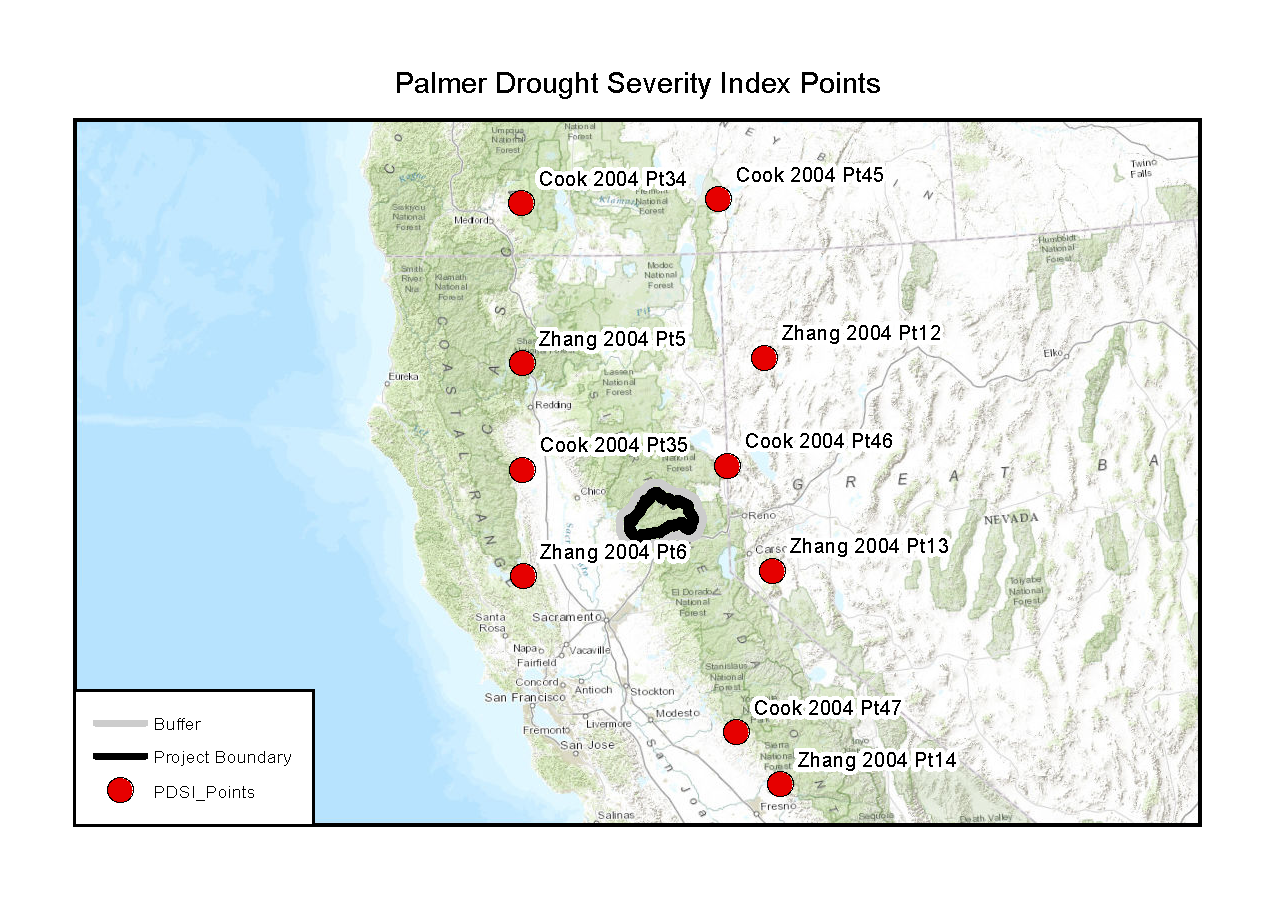
\includegraphics[width=\textwidth]{PDSIPointMap}
\end{figure}

\subsubsection{Calculations}
\begin{enumerate}
\item I combined all of the datasets into one Excel spreadsheet. 
\item Taking only the reconstructed data, I calculated the inverse distance weighted average of the PDSI values for each data point. 
\begin{enumerate}
\item Calculate the center point of the core area in ArcGIS.
\item Calculate the distance from each PDSI point to that center point. 
\item Rank the distances and standardize them by the closest point, such that the closest point is equal to 1 and the remaining points between 0 and 1. 
\item These effectively became the weight, and I calculated an overall average taking into account all of the weights by multiplying the PDSI value for a given year for each data point by this weighted value representing distance, summing them, and then dividing by the number of data points used. The number of data points used was not always the same because the Zhang data did not go as far back in time as the Cook data. 
\end{enumerate}
\item Convert yearly PDSI from 1550-1850 (historical period) into a 10-year average (PDSI per time step)
\item Recenter mean around 1 by rescaling 10-year PDSI values by 3-standard deviations: $y = \frac{x - \bar{x}}{2s + 1}$
\item Invert rescaled values so that positive values represent drought: $2\bar{x} - y$
\end{enumerate}

Finally, I created a comma-delimited text file containing only the time step values and the final PDSI values for import into RMLands.

\begin{figure}[h]
\centering
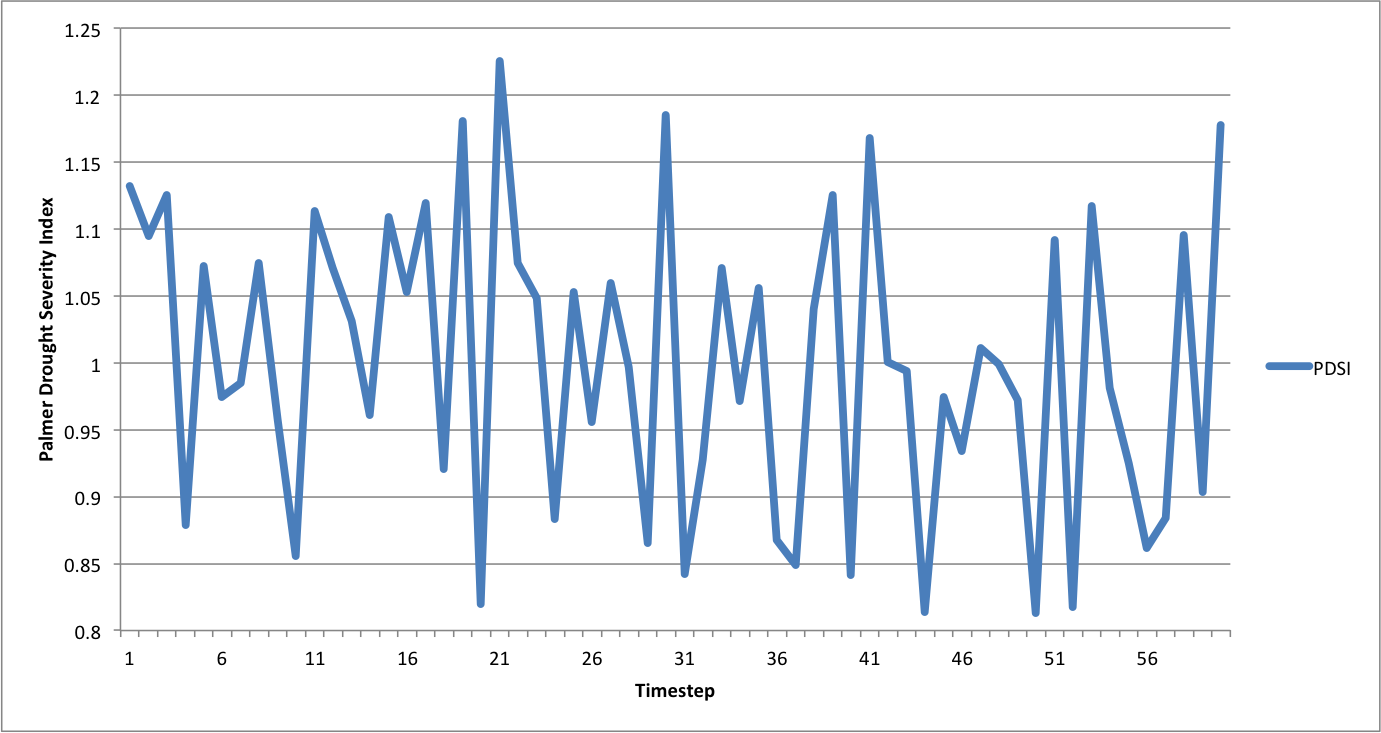
\includegraphics[width=0.8\textwidth]{PDSIpic}
\end{figure}

\subsection{Weather Stations}
I first looked into finding RAWS stations near the project area. Becky recommended using MesoWest, a service from the University of Utah that provides access to archived weather observations.

I consulted with a fuels specialist on the Tahoe as well as Becky in order to determine the dates of the fire season and hours for the daily burning period. On June 20th we resolved that fire season lasts from May 15 to October 15, and the burning period is 6-8 hours. Becky and I resolved to use 1000-1800 as the burning period.

Using MesoNet and Weather Underground, I identified several potential stations to use for weather data.
\begin{enumerate}
\item Rice Canyon (TT179): data going back to November 2012 
\item Saddleback: data going back to June 2001 (this is the station that gives the weather for Downieville, in the center of the project area)
\item Downieville [Wunderground] (KCADOWN12): data going back to 2009.
\item White Cloud: data going back to February 1993
\item Emigrant Gap: data going back to April 1997
\item Blue Canyon (KBLU): data going back to 1948
\end{enumerate}

From MesoWest, I downloaded data on the following variables:
\begin{itemize}
\item SKNT - wind direction in degrees
\item GUST - highest wind gust speed
\item DRCT - wind direction in categorial values (e.g. NW, SSE)
\item PEAK - highest sustained wind speed
\end{itemize}

\begin{figure}[h!]
\centering
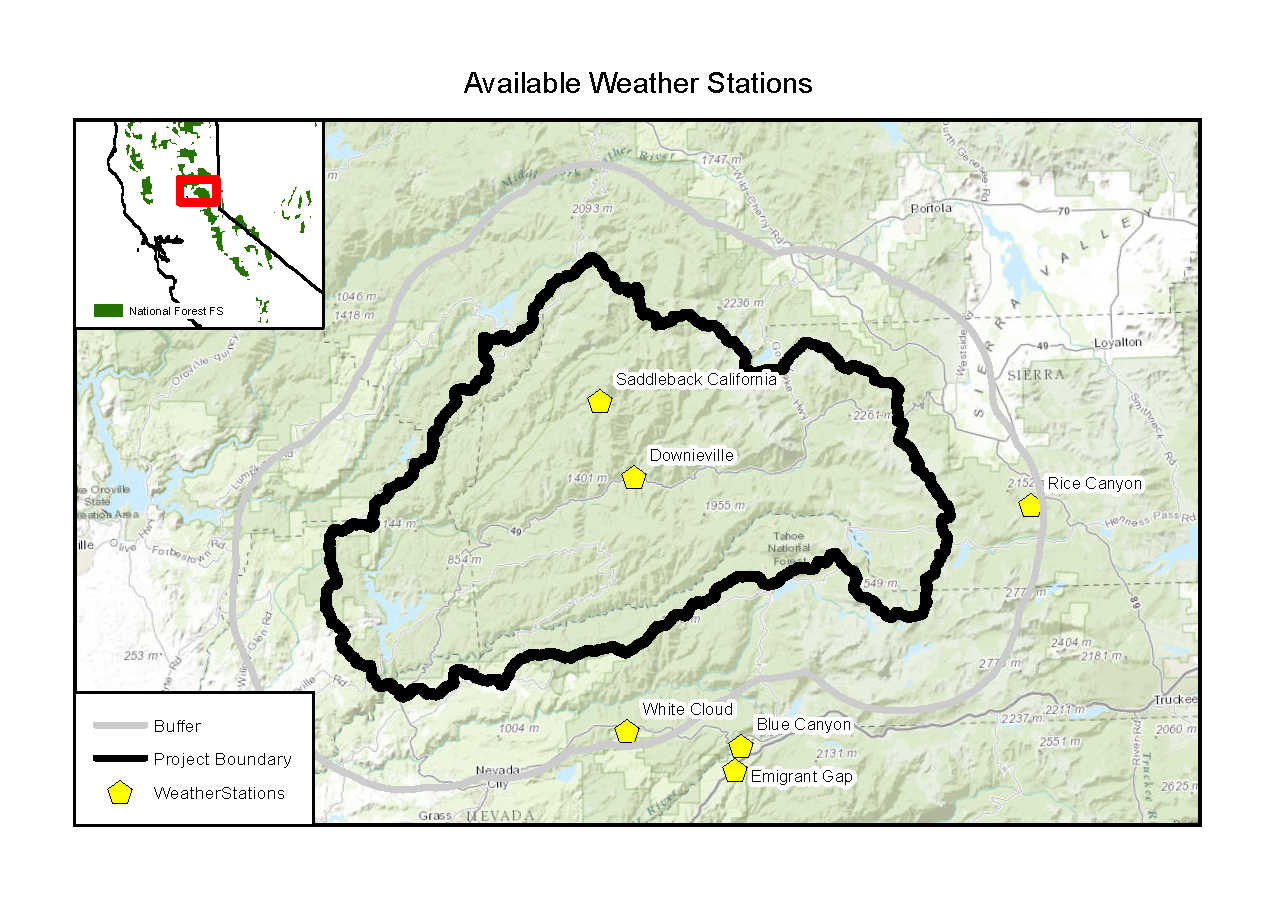
\includegraphics[width=\textwidth]{WeatherStationMap}
\end{figure}

Becky confirmed that all were close enough to the project area to be relevant.

The data for weather stations on Mesonet was obtained via a form for downloads on the mesonet website. I used a Python script to obtain the data stored on the Weather Underground site.
\begin{lstlisting}
import urllib2
#Create/open a file called wunder.txt (which will be a comma-delimited file), 
#in write mode
def weather(year):
#   works for 1948
    fname = '../Climate/WeatherStationData/wunder-data-%d.txt' % year
    f = open(fname, 'w')
    #Iterate through month, and day
    for m in range(5, 11):
        for d in range(1, 32):
            #Open wunderground.com url
            url = "http://www.wunderground.com/history/airport/KBLU/"+str(year)+"/" +str(m)+"/"+str(d)+"/DailyHistory.html?format=1"
            page = urllib2.urlopen(url)
            dailyData = page.read()
            f.write(dailyData)
    f.close()                            

#for year in range(1948, 1950):
#    weather(year)

def weather2(year):
#   works for 1949+
#   Create/open a file called wunder.txt (which will be a comma-delimited file), 
#   in write mode
    fname = '../Climate/WeatherStationData/wunder-data-%d.txt' % year
    f = open(fname, 'w')
    #Iterate through month, and day
    for m in range(5, 11):
        for d in range(1, 32):
            #Open wunderground.com url
            url = ''http://www.wunderground.com/history/airport/KBLU/'' + str(year) + ''/'' + str(m) + ''/'' + str(d) + ''/DailyHistory.html?req_city=NA&req_state=NA&req_statename=NA&format=1''
            page = urllib2.urlopen(url)
            dailyData = page.read()
            f.write(dailyData)
    f.close() 
\end{lstlisting}

I am primarily interested in the wind direction value, so even though there were many other data in each file, I created a new file storing only the wind direction data for the hours and dates in which I was interested.
\begin{lstlisting}
import glob
def wunderclean():
    ''' This function takes the output from the above functions and cleans it up so that it will only have the weather data from the hours that I will want it from. Range of times desired is 10:00 AM through 6:59 PM. The name of the first column (related to time of day) is inconsistent throughout the files. We have seen TimePDT, TimePST, and Time. We have decided not to convert TimePDT and PST to the same time. 'Time' seems to only appear once on a day in which the station malfunctioned and no data was recorded (June 6 1979). Another error arose from June 1998 in which the string printed ''No daily or hourly history data available,'' which we have corrected by adding 'No daily' to the list of cues to skip the line for data collection.
    '''
    outname = '../Climate/WeatherStationData/wunderclean.txt'
    #outname = '../Climate/WeatherStationData/'+ raw_input('new file name')
    out = open(outname, 'w')
    for fname in glob.glob('../Climate/WeatherStationData/wunder-data-*.txt'):
        print 'opening %s' %fname.split('/')[-1]
        f = open(fname, 'r')
        flines = f.readlines()
        for line in flines:
            if line.startswith('Time') or len(line) < 2 or line.startswith('No daily'):
                #print 'header or blank'
                continue
            elif not indaterange(line):
                #print 'out of range'
                continue
            hour = int(line.split(':')[0])
            if 10 <= hour < 12 and 'AM' in line:
                out.write(line)
            elif 12 == hour and 'PM' in line:
                # Special case Noon
                out.write(line)
            elif 1 <= hour <= 6 and 'PM' in line:
                out.write(line)
        f.close()
    out.close() 

def indaterange(line):
    """ Checks whether the line is from a date during the fire season. Currently only checks that the date is in May before May 15th (May 15th is OK)
    """
    baddates = [ '05-%02i' % i for i in range(15) ]
    for date in baddates:
        if date in line:
            return False
    return True

import glob
def mesonetclean(newfile, filepath):
    ''' This function takes the output from the above functions and cleans it up so that it will only have the weather data from the hours that I will want it from. Range of times desired is 10:00 AM through 6:59 PM
    '''
    outname = '../Climate/WeatherStationData/' + newfile
    #outname = '../Climate/WeatherStationData/'+ raw_input('new file name')
    out = open(outname, 'w')
    for fname in glob.glob('../Climate/WeatherStationData/'+ filepath):
        print 'opening %s' %fname.split('/')[-1]
        f = open(fname, 'r')
        flines = f.readlines()
        for line in flines:
            if line[0].isdigit():
                hour = int(line.split(',')[3])
                if 10 <= hour <= 18:
                    out.write(line)
                else:
                    continue
            else:
                continue
        f.close()
    out.close() 
\end{lstlisting}

Finally, I wrote a Python script to extract the wind direction in degrees from the downloaded weather data, bin it into categories, and generate the relative proportion on a 0-1 scale of wind direction.

\begin{lstlisting}
Bins for wind direction
(1) N [337.5-22.5 degrees]
(2) NE [22.5-67.5 degrees]
(3) E [67.5-112.5 degrees]
(4) SE [112.5-157.5 degrees]
(5) S [157.5-202.5 degrees]
(6) SW [202.5-247.5 degrees]
(7) W [247.5-292.5 degrees]
(8) NW [292.5-337.5 degrees]
(9) Flat [i.e., slope = 0]
(NODATA) cells outside of project boundary

===============================================================
import numpy as np

#variables

windN = 0
windNE = 0
windE = 0
windSE = 0
windS = 0
windSW = 0
windW = 0
windNW = 0
windFLAT = 0
windcounts = { d : 0 for d in ['N','NE','E','SE','S','SW','W','NW'] }

kbludata = np.genfromtxt("WeatherStationData/wunderclean.txt", dtype=int, delimiter = ',', skip_header = 1, usecols = 12) 

#note for mesowest variables DRCT is the wind direction
slecdata = np.genfromtxt("WeatherStationData/SLEC1.txt", dtype=int, delimiter = ',', usecols = 8, missing_values='', filling_values='0') 
ciscdata = np.genfromtxt("WeatherStationData/CISC1.txt", dtype=int, delimiter = ',', usecols = 8, missing_values='', filling_values='0') 
#slecdata_save = np.savetxt("WeatherStationData/SLEC1_WindSpd.txt", slecdata, delimiter=',')

for item in kbludata:
    winddir = item
    if (winddir > 337.5) or (winddir <= 22.5) & (winddir > 0):
        windN += 1
    elif (winddir > 22.5) and (winddir <= 67.5):
        windNE += 1
    elif (winddir > 67.5) & (winddir <= 112.5):
        windE += 1
    elif (winddir > 112.5) & (winddir <= 157.5):
        windSE += 1
    elif (winddir > 157.5) & (winddir <= 202.5):
        windS += 1
    elif (winddir > 202.5) & (winddir <= 247.5):
        windSW += 1
    elif (winddir > 247.5) & (winddir <= 292.5):
        windW += 1
    elif (winddir > 292.5) & (winddir <= 337.5):
        windNW += 1
    elif (winddir == 0):
        windFLAT += 1
    else:
        print "Wind direction not an allowed value."    
print "Totals after KBLU:"
print "windN =", windN, "windNE =", windNE, "windE =", windE, "windSE =", windSE, "windS =", windS, "windSW =", windSW, "windW =", windW, "windNW =", windNW, "windFLAT =", windFLAT

for item in slecdata:
    winddir = item
    if (winddir > 337.5) | (winddir <= 22.5) & (winddir > 0):
        windN += 1
    elif (winddir > 22.5) & (winddir <= 67.5):
        windNE += 1
    elif (winddir > 67.5) & (winddir <= 112.5):
        windE += 1
    elif (winddir > 112.5) & (winddir <= 157.5):
        windSE += 1
    elif (winddir > 157.5) & (winddir <= 202.5):
        windS += 1
    elif (winddir > 202.5) & (winddir <= 247.5):
        windSW += 1
    elif (winddir > 247.5) & (winddir <= 292.5):
        windW += 1
    elif (winddir > 292.5) & (winddir <= 337.5):
        windNW += 1
    elif (winddir == 0):
        windFLAT += 1
    else:
        print "Wind direction not an allowed value."    
print "Totals after KBLU, SLEC:"
print "windN =", windN, "windNE =", windNE, "windE =", windE, "windSE =", windSE, "windS =", windS, "windSW =", windSW, "windW =", windW, "windNW =", windNW, "windFLAT =", windFLAT

for item in ciscdata:
    winddir = item
    if (winddir > 337.5) | (winddir <= 22.5) & (winddir > 0):
        windN += 1
    elif (winddir > 22.5) & (winddir <= 67.5):
        windNE += 1
    elif (winddir > 67.5) & (winddir <= 112.5):
        windE += 1
    elif (winddir > 112.5) & (winddir <= 157.5):
        windSE += 1
    elif (winddir > 157.5) & (winddir <= 202.5):
        windS += 1
    elif (winddir > 202.5) & (winddir <= 247.5):
        windSW += 1
    elif (winddir > 247.5) & (winddir <= 292.5):
        windW += 1
    elif (winddir > 292.5) & (winddir <= 337.5):
        windNW += 1
    elif (winddir == 0):
        windFLAT += 1
    else:
        print "Wind direction not an allowed value."    
print "Totals after KBLU, SLEC, CISC:"
print "windN =", windN, "windNE =", windNE, "windE =", windE, "windSE =", windSE, "windS =", windS, "windSW =", windSW, "windW =", windW, "windNW =", windNW, "windFLAT =", windFLAT

==============================================================

RESULTS At 1612 on 8/23/2013:
Totals after KBLU, SLEC, CISC:
windN = 3612 windNE = 4616 windE = 5340 windSE = 6039 windS = 33015 windSW = 26450 windW = 25230 windNW = 6420 windFLAT = 10262

============================================

windarray = [3612., 4616., 5340., 6039., 33015., 26450., 25230., 6420.]
windsum = sum(windarray)
windpercent = divide(windarray, windsum)
[ 0.03262224  0.04169     0.0482289   0.05454201  0.29817922  0.23888658  0.22786799  0.05798306]

 N 0.03262224
 NE 0.04169
 E 0.0482289
 SE 0.05454201
 S 0.29817922
 SW 0.23888658
 W 0.22786799
 NW 0.05798306
\end{lstlisting}

\section{Fire Size}
To calculate the proportion of fires within a set of bins ordered by magnitude (1, 10, 100, 1,000, 10,000, and 100,000 hectares), I used real data. Data on fire sizes in California goes back to approximately 1904 in the state. However, I did not want to use fire sizes from the entire state, since it is so large and encompasses so many diverse ecosystems. The Existing Vegetation layers were developed for the whole state as well, and published in subsections by ecotype. One of those ecotypes is the North Sierra, also known as Zone 3. The CalVeg alliances were tied to this zone as well. I then used the Pacific Crest Trail as a conservative eastern boundary (the trail is often to the east of the actual crest in the study landscape), redrawing the polygon. I then clipped the fire occurrence data to the new polygon, and sorted the fires using a python script.

\begin{lstlisting}
point = np.genfromtxt("point_table_0923_1743.txt", delimiter=',', skip_header=1, usecols=30, comments=None)
poly = np.genfromtxt("poly_table_0923_1743.txt", delimiter=',', skip_header=1, usecols=15, comments=None)
both = np.append(point, poly)
both_ha = both * 0.404686
bins = [0, 1, 10, 100, 1000, 10000, 100000]
\end{lstlisting}



The output of the histogram function gives the number of fires falling within each size range.
\begin{lstlisting}
In: np.histogram(both_ha, bins=bins)
Out: 
(array([8107,  609,  460,  398,  102,   13]),
 array([     0,      1,     10,    100,   1000,  10000, 100000]))
\end{lstlisting}

Finally, I computed the proportion of fires in each bin.
\begin{lstlisting}
binnedfire, bins = np.histogram(both_ha, bins=bins)
In: rml_firevals = binnedfire / np.sum(binnedfire, dtype=np.float)
Out: array([ 0.83672206,  0.06285478,  0.04747652,  0.04107751,  0.0105274 , 0.00134173])
In: rml_firevals_pct = rml_firevals * 100
Out: array([ 83.67220559,   6.28547838,   4.74765198,   4.10775106, 1.05274022,   0.13417277])
\end{lstlisting}        

\section{Susceptibility}
\subsection{Hazard Function}
One input in the model is to apply the hazard function of the Weibull model to the susceptibility to fire for a given cover type. The inputs are scale (equivalent to mean FRI), shape (which has no deterministic basis, and is typically 3), and the reset point for the function (age since any disturbance, age since high mortality, age since low mortality, age since condition class change, etc). There is an accompanying graphic within RMLands that shows what this curve looks like for a given cover type parameter selection. While we were parameterizing the adapted model the first time, Kevin realized that prior uses of the model had technically misused the hazard function, which is an unbounded on the right function. In previous versions, RMLands simply truncated the hazard function when the output value reached 1 (because it is treated as a probability in the model). It did not cause problems in prior runs, but appeared to in our initial Sieran runs. Consequently, we will modify RMLands such that in future simulations the cumulative form of the Weibull model will be used instead. It contains the same parameters as the hazard.

For at least the initial parameterization of the model, we used the expert and literature-generated FRI values. When choosing ``age since \_\_\_\_\_\_,'' we selected ``Age since any disturbance'' for fuel-driven cover types, and ``Age since high mortality disturbance'' for climate and weather-drive cover types.

\subsection{Spread Weights}
Where the model asks for inputs for Min and Max, this refers to fire size. Recall that each fire is probablistically assigned a maximum size at the time of initiation. Reviewing the fire size distribution for most areas reveals that most fires fall on the ``min'' side.

\section{Spread}
Use joint cell: if multiple adjacent burning cells, a given unburnt cell is more likely to burn. it get evaluated multiple times and the probabilities are summed.
Cell evaluation: cells are reevaluated each step
Majority filter - 3x3 window to smooth fire edges and fill in holes
Local spread window: to deal with pixelated landscapes - mostly for bugs


          
\chapter{Model Calibration}
General note: when exporting output data, they go to the main folder for the run executed and are simply appended to the existing csv files, so they do not have to be moved around, and this is also how you can compare multiple runs of the simulation in one R function. 

\section{Check that disturbance and succession rules executed}
In R, run script to generate drulecheck.csv and srulecheck.csv. These files show the number of eligible pixels for each rule over the course of the entire simulation, and the number of pixels that were subjected to each rule. If the probability of a given rule was 1, then all eligible pixels should have been subjected to the rule. If the probability was less than one, than the percentage of pixels subjected to a rule should be equivalent to the probability of that rule being executed.

\section{Preturn vs. SReturn}
Pixel return vs. Stand return? Preturn shows cell-level return interval (the ideal) while sreturn shows the average for all cells of that cover type. Note, still not sure how these differ from rotation.

\section{Susceptibility}
In order to differentiate open conditions from closed conditions, parameterization of susceptibility in RMLands must be done by assigning single susceptibility values to each condition class for a cover type, rather than use the Weibull function. I calculated relative susceptibility among the conditions for given cover types based on the LandFire values. However, we were not sure how to convert these values into the susceptibility numbers. I began by using the actual relative values (which summed to 1), but these resulting in not enough fire in the types for which this was used (SMC and RFR).

\section{Specific Run Results}

\subsection{October 7}
Increased susceptibility of non-Hazard Function types by 0.5

\paragraph{darea}: 5-88\%: probably too much fire for Tahoe folks
\paragraph{rotation}: 
\begin{itemize}
\item CMM - too low
\item LPN - too much any
\item LPN\_ASP - too much any
\item MHW: not enough any
\item MHW\_U: not enough any
\item MRIP: too much any
\item OAK: not enough any
\item OCFW: not enough any (right proportions)
\item OCFW\_U: not quite enough
\item RFR: too short
\item SMC\_M: good
\item SMC\_X: too long
\item SMC\_U: too short
\item SMC\_A: little too short
\item SCN: too short
\end{itemize}

\paragraph{rulechecks}: Both ok

\paragraph{Thoughts} Extra fire is likely due to so much in early. If early is fairly susceptible then a cover type may get stuck in it. One solution would be to allow low mortality in early seral, although this goes against our understanding of early seral fire. Another thing we can do is reduce the percentage/likelihood of high mortality fire. Another thing to do would be to consider chaparral as a landscape component - is the amount in it reasonable? Its fire recurrence? It's possible that our gut feelings are driven by the knowledge of Rocky Mountain systems and need to be adjusted. This would be a good subject for discussion with Becky and the other Tahoe folks. 

 

\backmatter 
\include{glossary} 
\include{notat} 
\bibliographystyle{amsalpha} %The style you want to use for references. 
\bibliography{mr,refs} %The files containing all the articles and books you ever referenced. 
%\printindex %Make an index AUTOMATICALLY 

\end{document} 